\section{Test}

%Lav mindst tre testcases med tilhørende fremgangsmåde/testprocedure og testrapporter.
%Lav mindst én Junit test til centrale metoder. Inkludér code coverage dokumentation.
%Lav mindst én brugertest. Husk at brugeren skal være en der ikke kan kode.

\subsection{Programtest}


\subsection{Brugertest}

\subsection{Test af terningens tilfældighed}
    \begin{figure}[H]
        \centering
        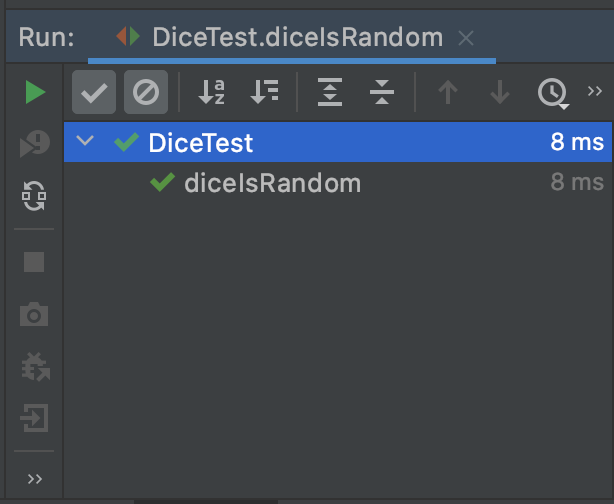
\includegraphics[width=8cm]{figures/diceIsRandomTest.png}
        \caption{JUnit test for at teste tilfældigheden af Dice klassens metode roll()}
        \emph{Testen af Dice klassen og dens roll() metode var en succes. Koden ses i bilag \ref{diceTest}}
    \end{figure}
    

\subsection{Test af chancekort tilfældighed}
    \begin{figure}[H]
        \centering
        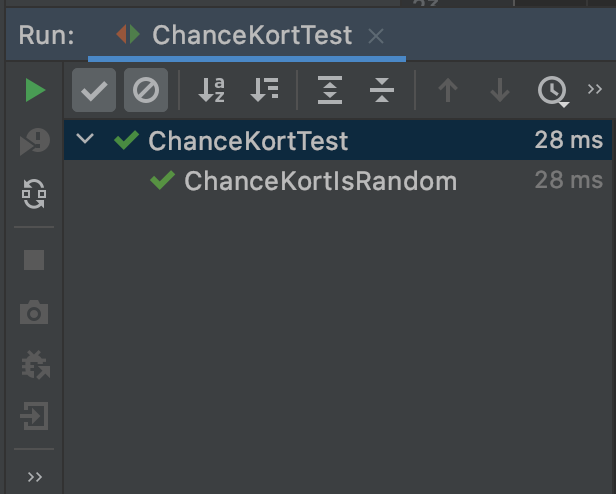
\includegraphics[width=8cm]{figures/chanceKortIsRandom.png}
        \caption{JUnit test for at teste tilfældigheden af ChanceKort klassens metode randomChanceKort()}
        \emph{Testen af ChanceKort klassen og dens randomChanceKort() metode var en succes. Koden ses i bilag \ref{ChanceKortTest}}
    \end{figure}
    
    
    \subsection{Test af antal chancekort}
    \begin{figure}[H]
        \centering
        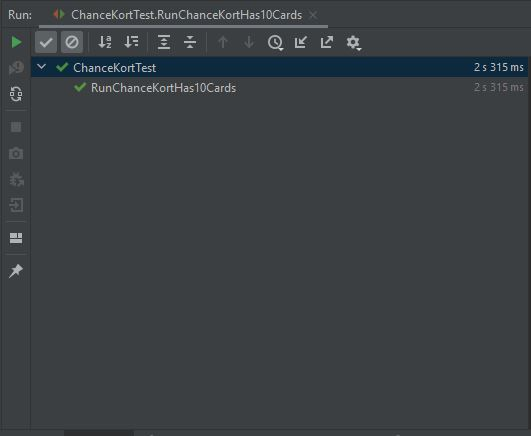
\includegraphics[width=15cm]{figures/RunChanceKortHas10Cards.JPG}
        \caption{JUnit test for at teste at RunChanceKort klassen indeholder det rigtige antal kort.}
        \emph{Testen af RunChanceKort klassen var en succes. Koden ses i bilag \ref{ChanceKortTest}}
    \end{figure}





